\begin{figure}[tbh]
\centering
\setlength{\abovecaptionskip}{0pt plus 3pt minus 2pt}
\setlength{\belowcaptionskip}{-10pt plus 3pt minus 2pt}
\caption*{}

% \includegraphics[width=.9\linewidth]{./images/rebutall_2cams.jpg}
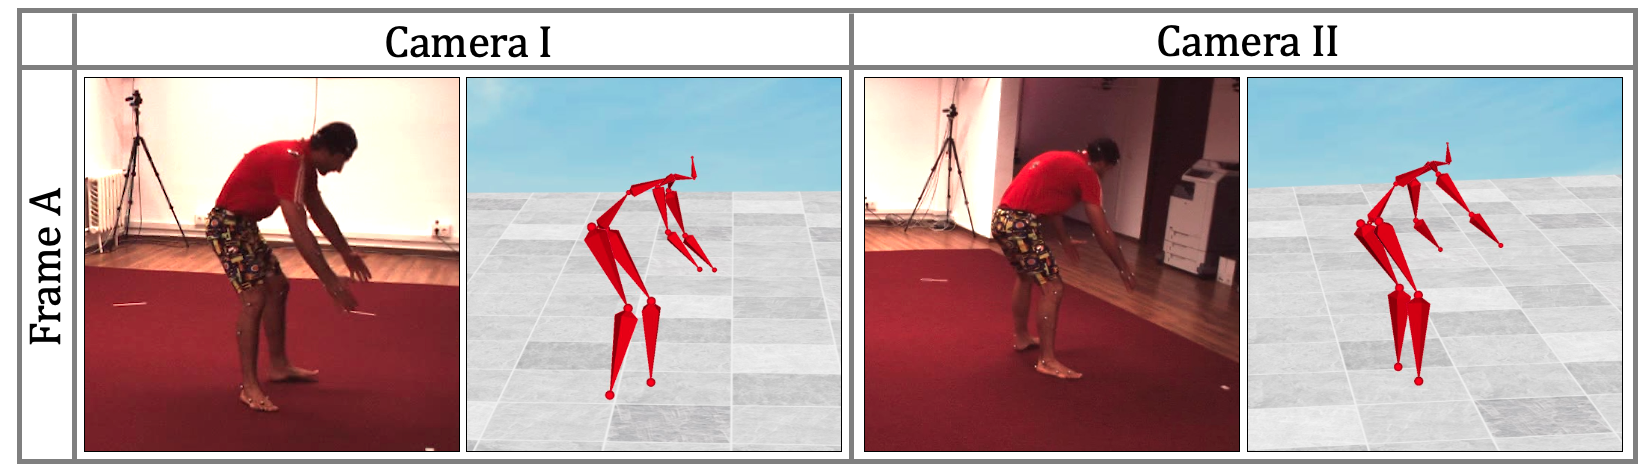
\includegraphics[width=.9\linewidth]{./images/rebutall_2cams_b.png}

\setlength{\abovecaptionskip}{-10pt plus 3pt minus 2pt}
\setlength{\belowcaptionskip}{-20pt plus 3pt minus 2pt}

\caption{
%Generalization: 
Evaluation on two cameras, while training on two others.}
% (a) evaluation on the Ski-pose dataset. (b) evaluation on 2 cameras, while training on 2 others.}
\label{fig:general}

\end{figure}